
\section{Other Concepts}
\textit{Overfitting}: Occurs when the cost in the training dataset decreases but it increases on the test dataset. The model starts to \textit{memorize} data, and does not \textit{generalize}.

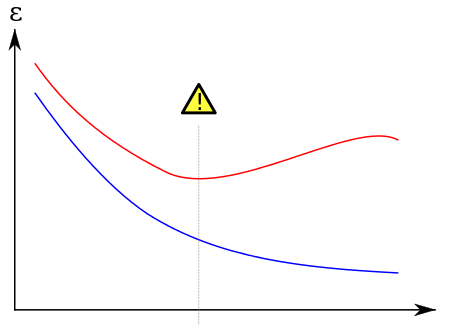
\includegraphics[width=\textwidth]{overfitting.png}

Training error: blue; validation error: red, both as a function of the number of training cycles. The best predictive and fitted model would be where the validation error has its global minimum.

\textit{Underfitting}: It occurs when the model or algorithm does not fit the data enough. It could be a bad model (too simple, or just not the right fit), or a lack of training, etc.

\textit{Classification v Regression}: A classification model is one which attempts to predict a class, or category. That is, it's predicting from a number of discrete possibilities, such as "dog" or "cat." A regression model is one which attempts to predict one or more numeric quantities, such as a temperature or a location. Which one we use depends on the nature of the variables.

\textit{Cross Validation}: The goal of cross-validation is to test the model's ability to predict new data that was not used in estimating it, in order to flag problems like overfitting or selection bias, and to give an insight on how the model will generalize to an independent dataset.

Why a CNN? It's the current state-of-the-art approach to creating computer vision models.

\section{High Level View}
Deep Learning is a Machine Learning area. The latter can be associated with the image, where update maps to learning in human terms, and more data maps to more experience (in human life). A program that learns from experience.

\begin{figure}
 \centering
 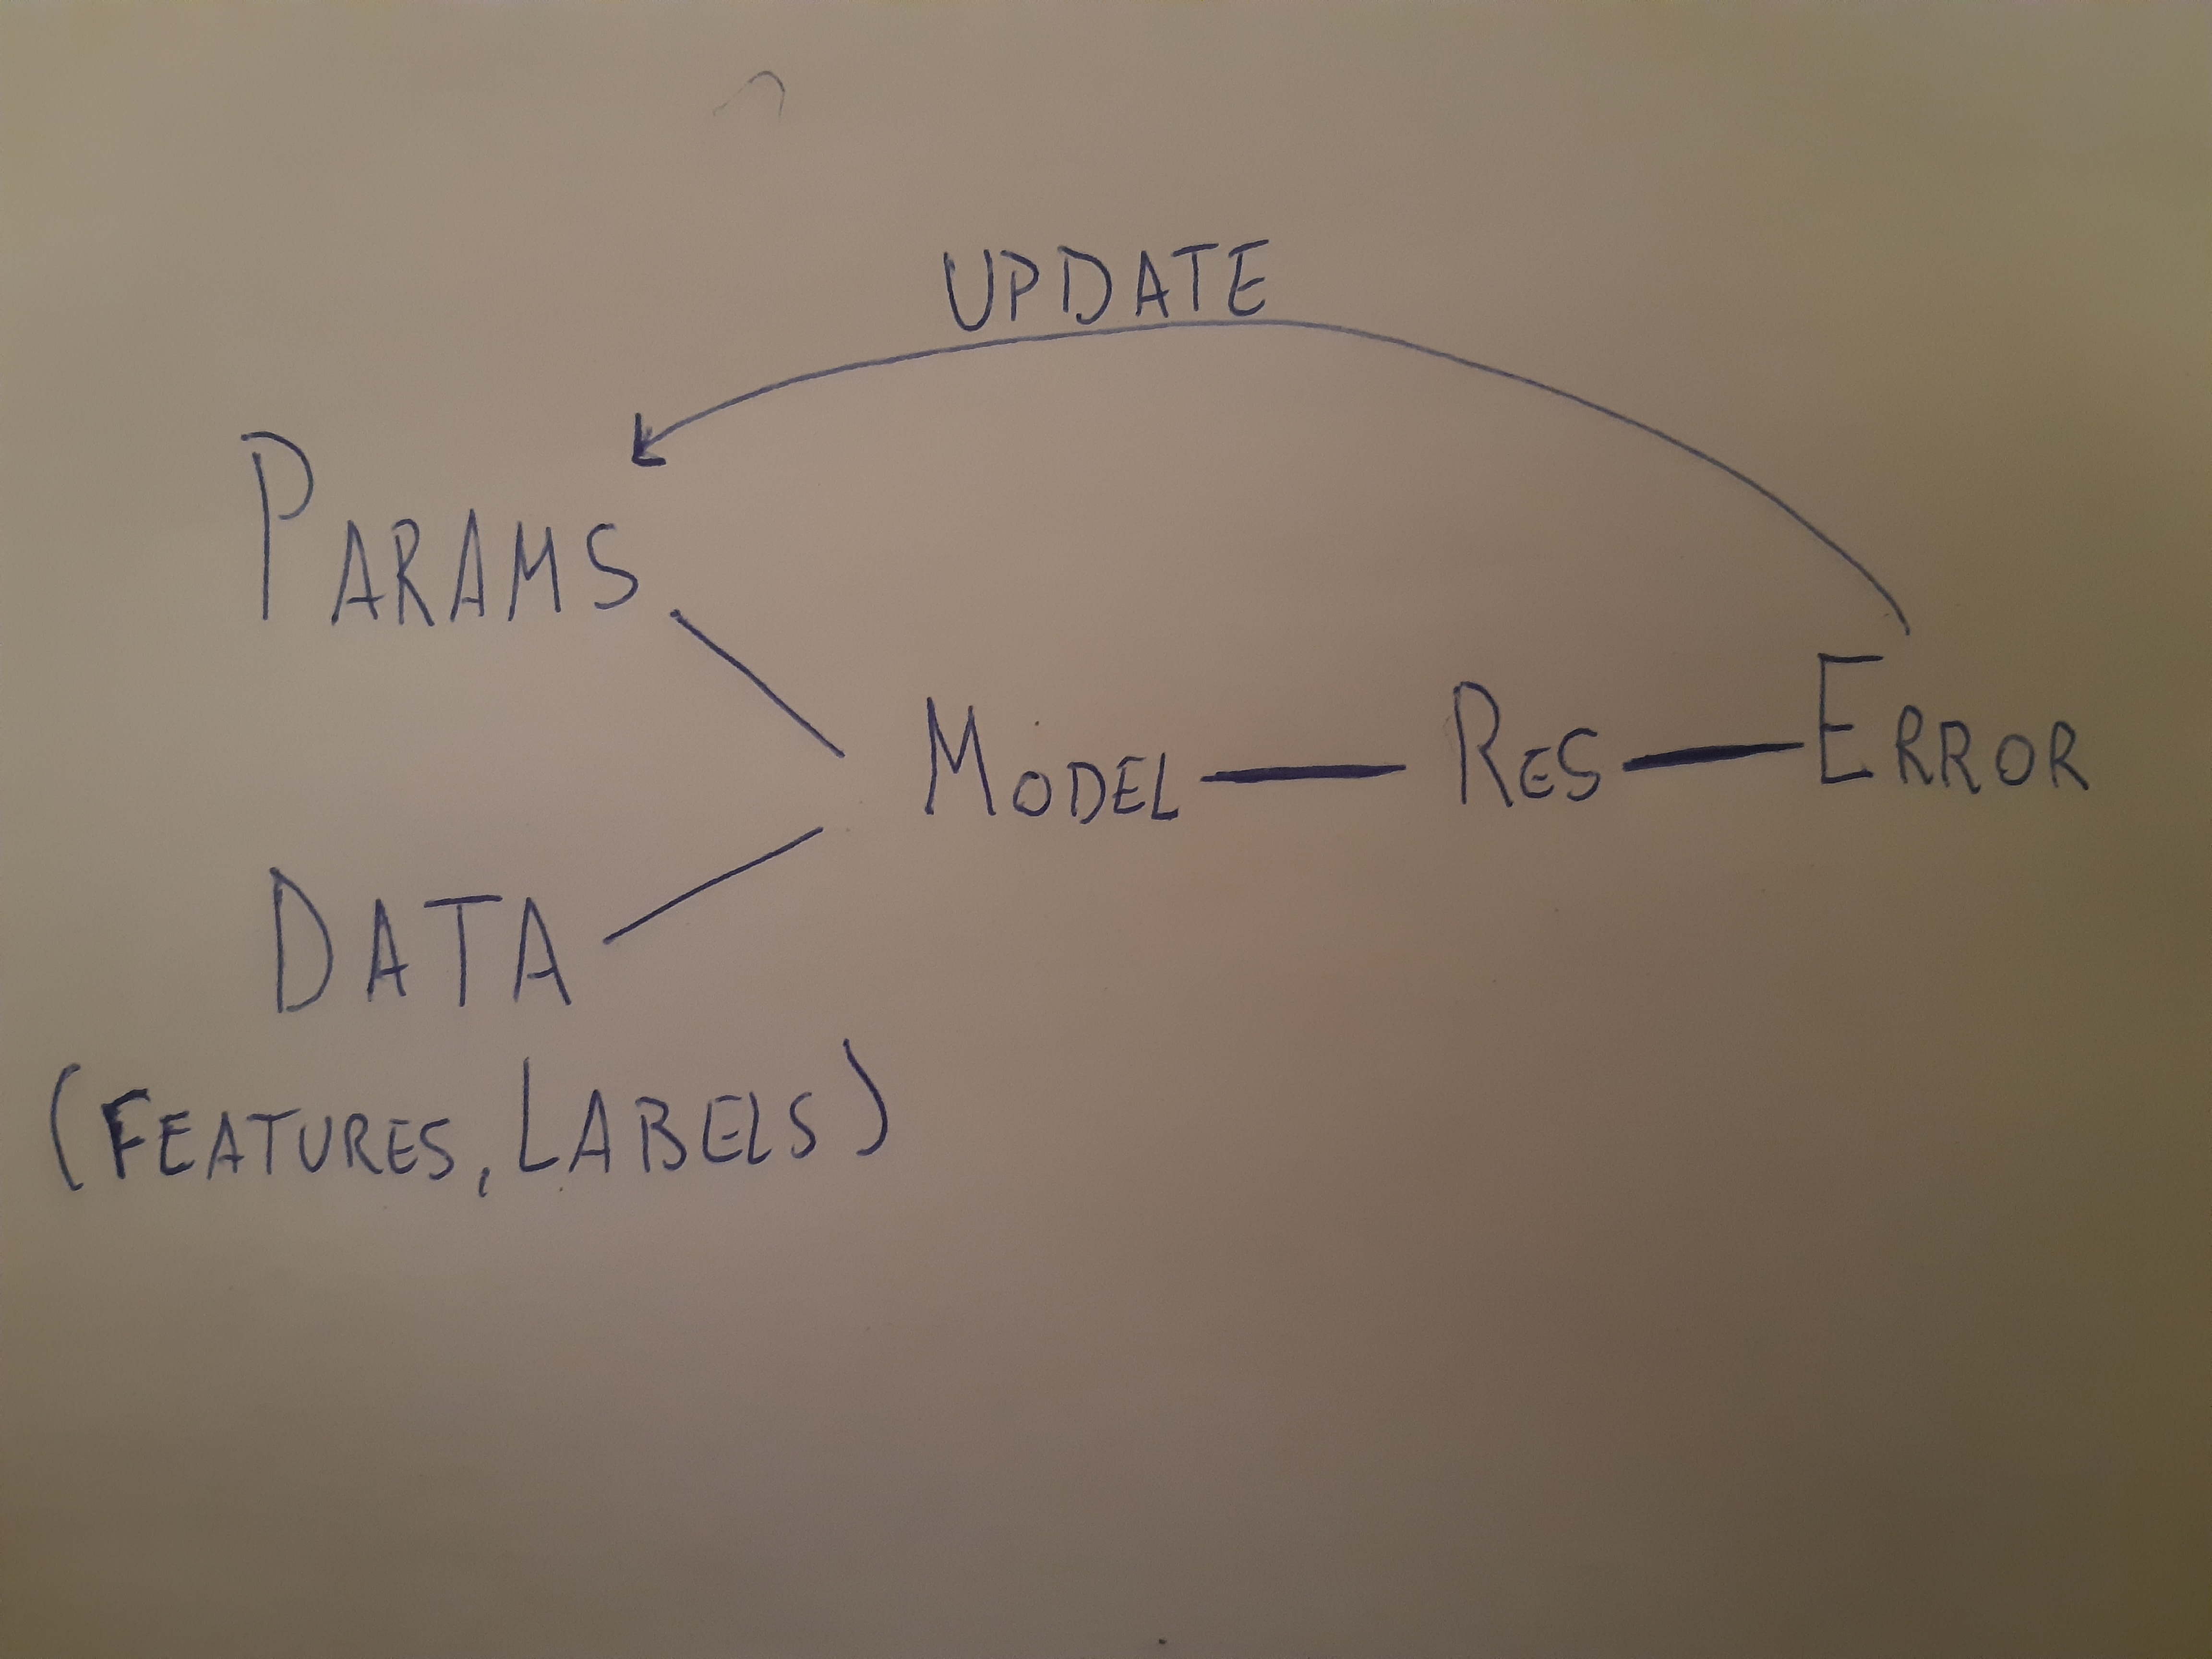
\includegraphics[width=0.9\textwidth]{ML.jpg}
 \caption{Machine Learning Process}
\end{figure}


\begin{figure}
 \centering
 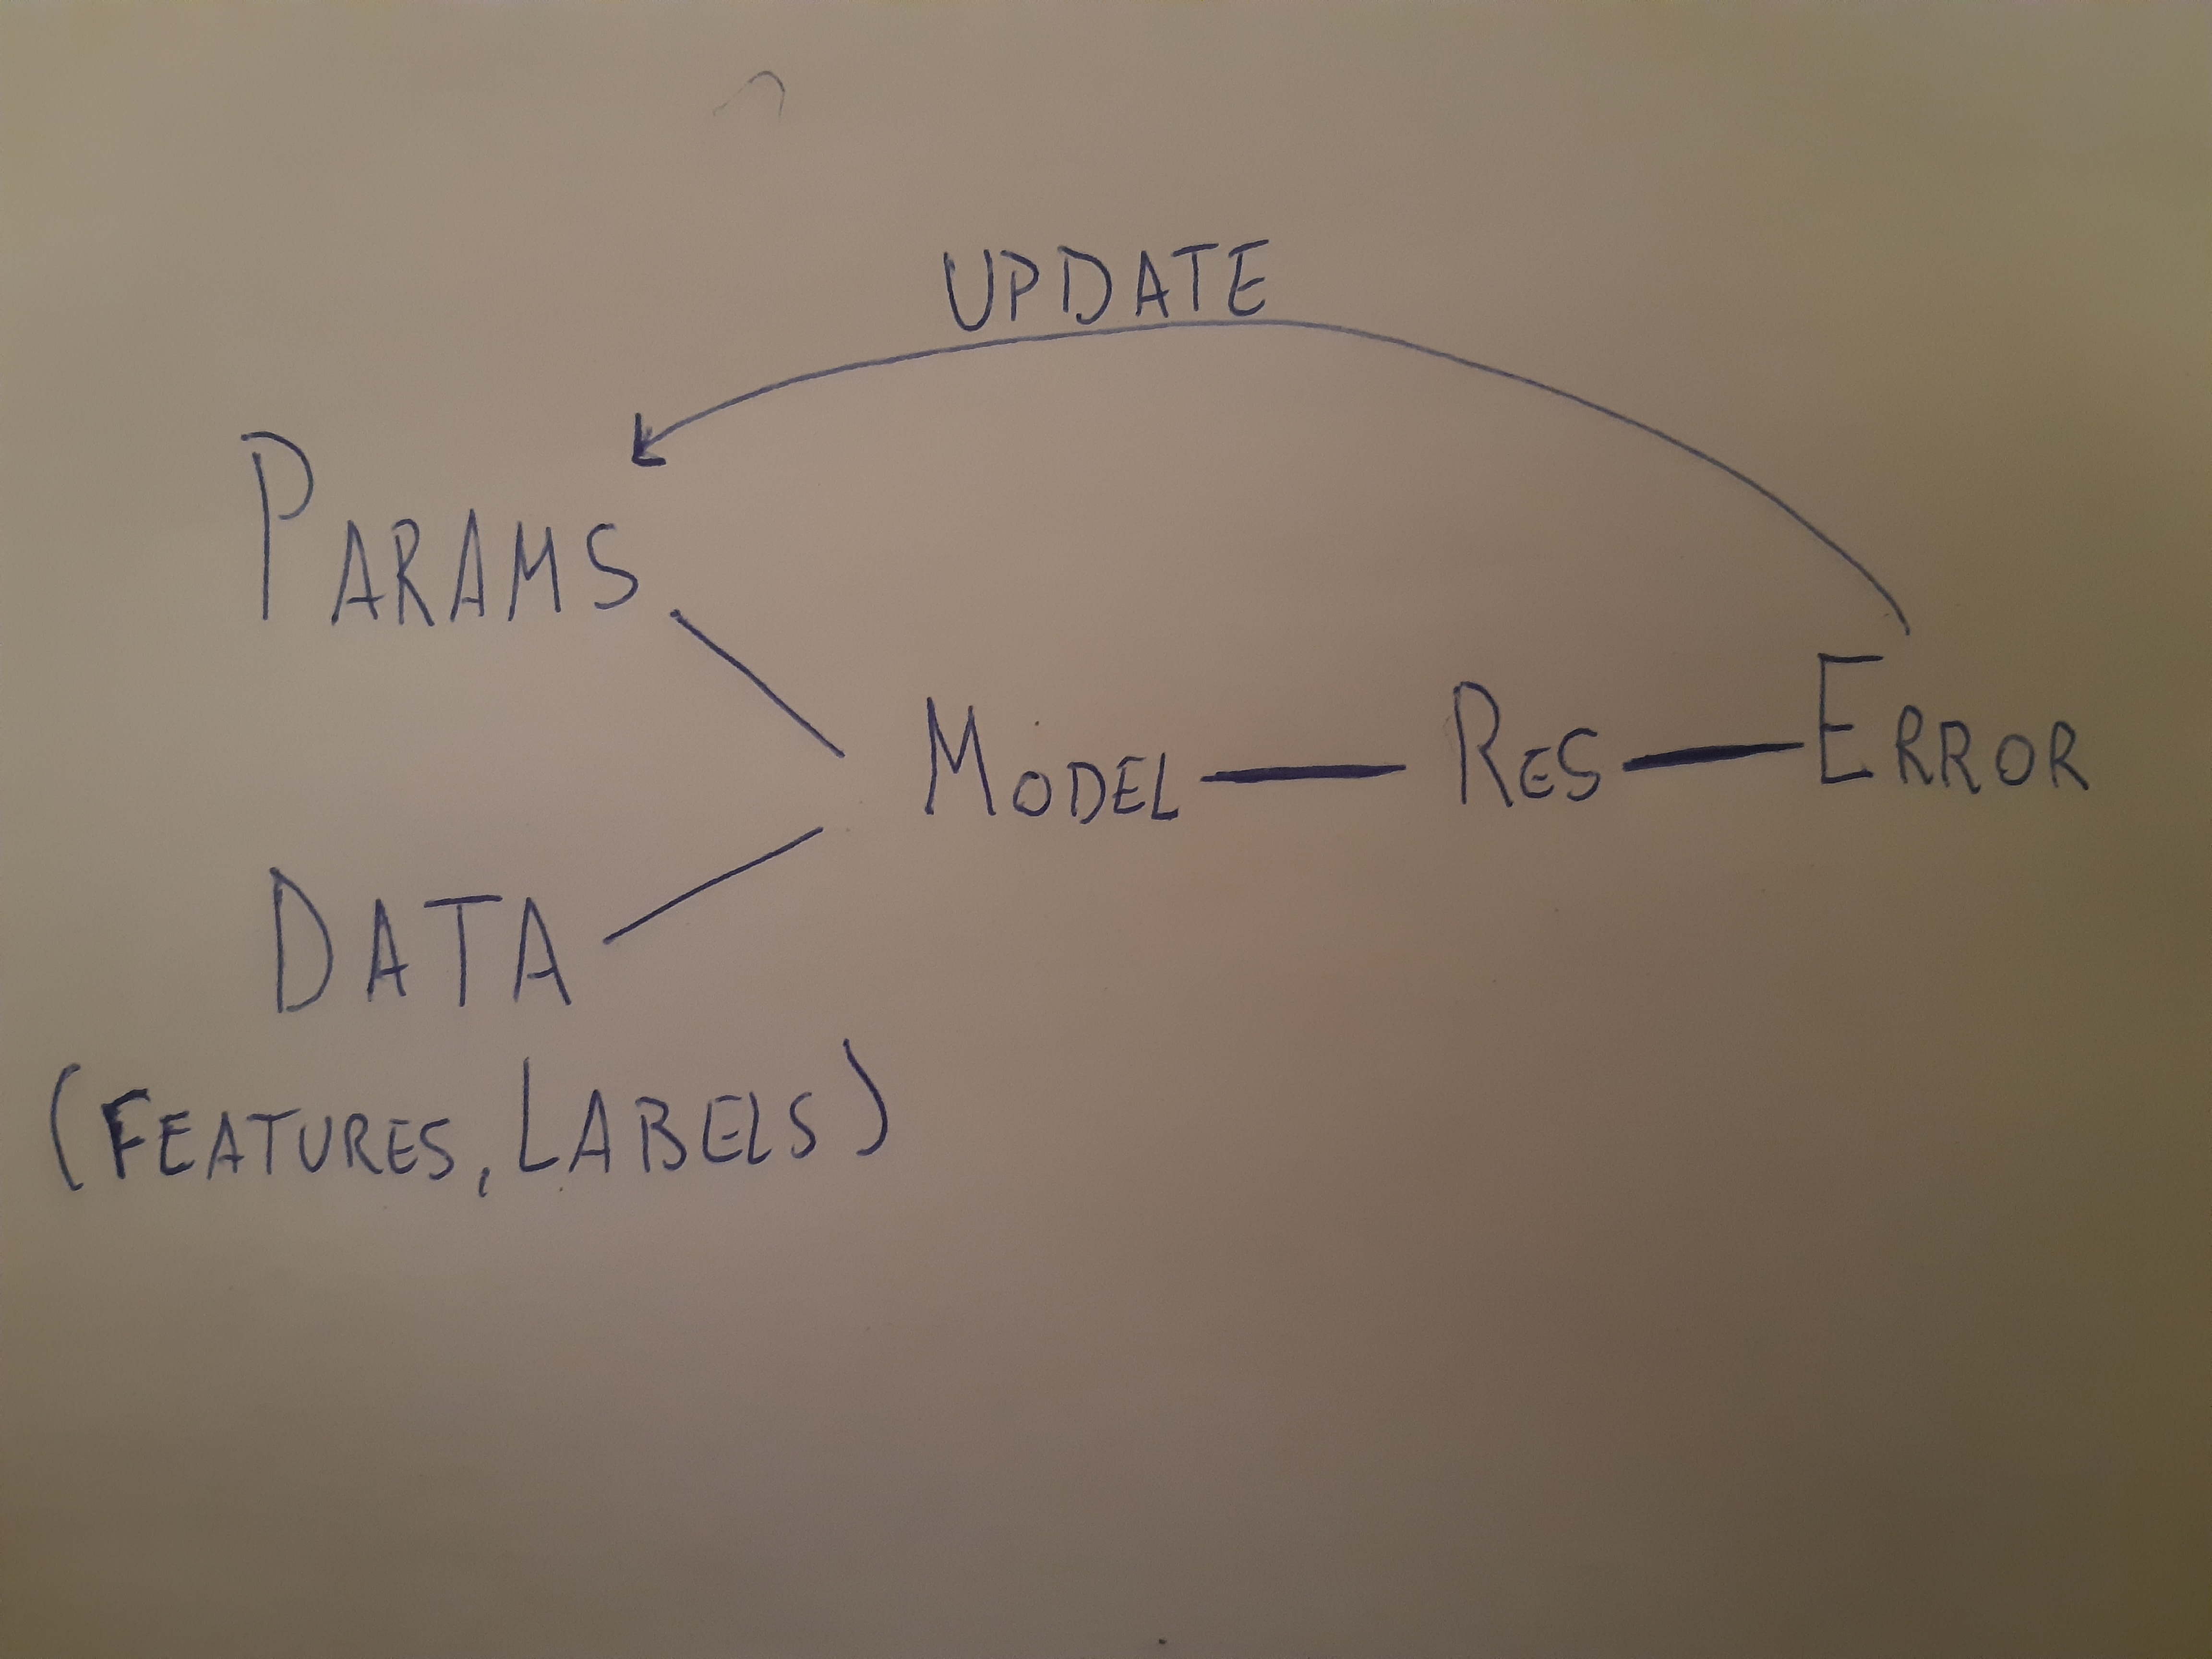
\includegraphics[width=0.9\textwidth]{ML.jpg}
 \caption{Two Layer NN}
\end{figure}

